\chapter{Proposed Methodology and Paradigm}\label{chap:methodology}
Founded on the vision outlined in the requirements specification (Chapter~\ref{chap:req}), this research aims to propose a novel system that combines the strengths of 
classical Graph-based architectures with the generative capabilities of Large Language Models (LLMs). This chapter details the foundational methodology of our system. 
\section{Overview}
The proposed paradigm can be construcuted and visualized as the below pipeline
\begin{figure}[H]
    \centering
    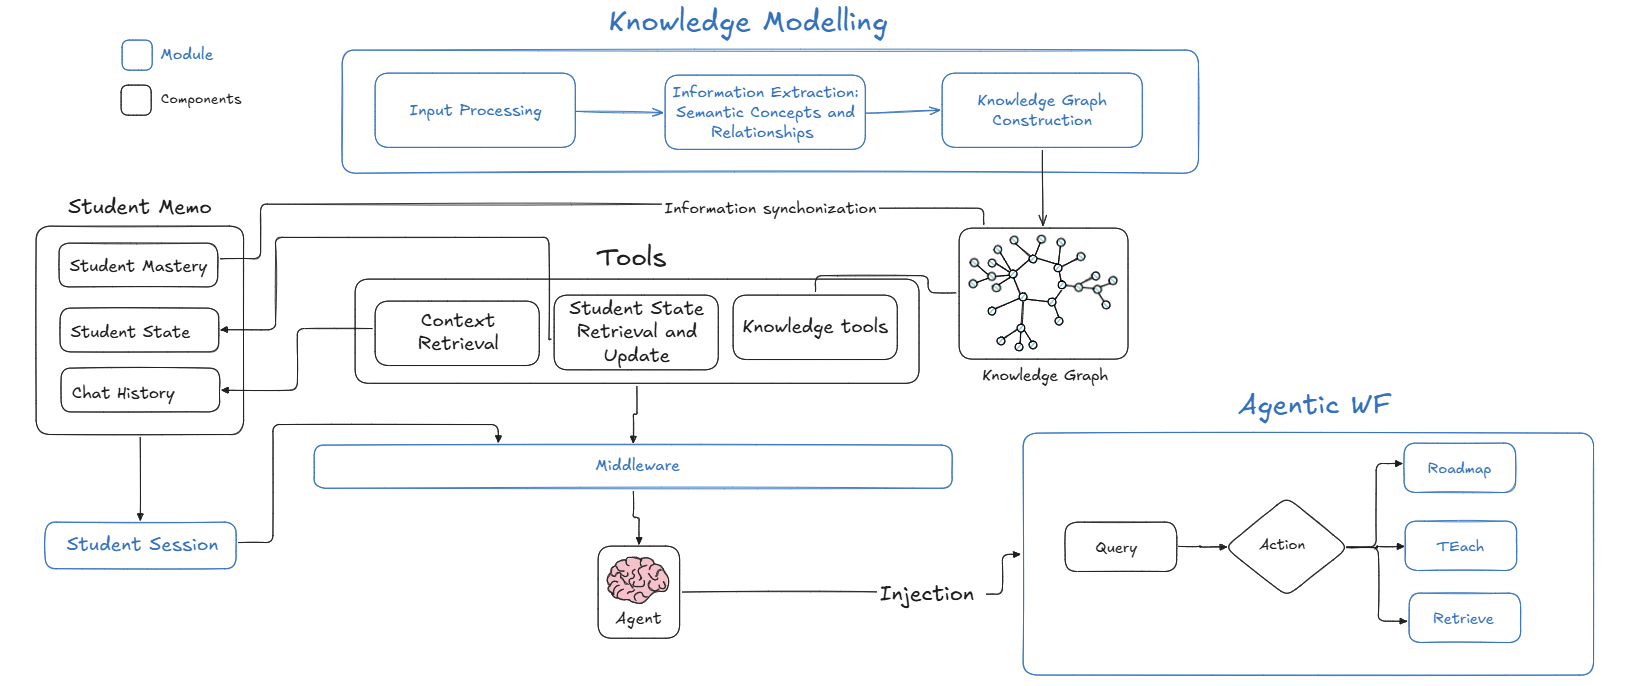
\includegraphics[width=\textwidth]{Images/method/pipeline.png}
    \vspace{12pt}\caption{High level visualization of how the system should work}\label{fig:macro_workflow}
\end{figure}

A key security boundary is established at the system's entry point. Upon user authentication, the student's Session and Memo contexts are directly injected into the 
computational tools. As a result, the agents use these pre-configured tools instead of interacting directly with the database. This approach ensures strict data 
isolation and prevents the LLM from making unauthorized or destructive database transactions.

\section{Knowledge Modelling: Educational Graph}
This section proposes a hybrid methodology that anchors the generative flexibility of LLMs to the deterministic rigor of Graph Construction and Natural Language Processing. 
By formulating the educational domain as a Property Graph, the proposed system (SmartEdu) achieves a necessary synthesis of semantic richness and logical consistency, 
overcoming the unstructured chaos often associated with pure generative models.
\subsection{Graph Definition}\label{sub:g_def}
To construct a graph, we need to define and regulate it with a connected, rigorous structure. Simulating educational concepts, the graph contains ontologies as well as 
topic's relationship like presiquite. The subsequence contents in this subsection explain the deterministic algebra representation and rules explanation of it.
\subsubsection{Formal Property and Topological Definition}

To accurately represent the vast, interconnected semantic structure inherent in educational curricula, our methodology employs a formal Property Graph formulation. Unlike simple directed graphs, a property graph allows both vertices and edges to possess complex internal states (properties). This multidimensionality is highly suitable for educational knowledge representation, where a concept is not just a node, but a container of definitions, mathematical formulas, and historical context.

We define the Educational Knowledge Graph (EKG) as a heterogeneous, directed property graph, formally denoted as:
\begin{equation}
    G = (V, E, \Lambda, \Pi)
\end{equation}
where:
\begin{itemize}
    \item $V$ is the set of vertices (nodes), representing distinct educational entities spanning multiple levels of abstraction.
    \item $E \subseteq V \times V$ is the set of directed edges, representing the semantic and structural relationships between entities.
    \item $\Lambda$ is a finite, predefined set of labels, acting as ontological categories that strictly classify the nodes to prevent semantic drift.
    \item $\Pi$ is a set of properties, expressed as key-value pairs $\pi_{key} = value$, associated with both nodes and edges to store metadata, raw textual content, and dynamically updated quantitative metrics.
\end{itemize}

The necessity of this mathematical definition lies in its ability to enforce data integrity. By treating the knowledge base as a set $V$ and a mapping $E$, we can apply rigorous graph-theoretic algorithms (such as topological sorting and shortest-path routing) directly to the curriculum, effectively translating human pedagogical intuition into computationally solvable problems.

\subsubsection{Ontological Hierarchy formulation}

To accurately model the multi-scalar nature of educational curricula—ranging from entire academic disciplines down to specific explanatory sentences in a textbook—we artificially constrain the label set $\Lambda$ such that $\Lambda = \{ \text{CommunityNode}, \text{TopicNode}, \text{ConceptNode}, \text{RhetoricalNode} \}$. This rigorous ontological taxonomy ensures structural consistency across different domains:

\begin{itemize}
    \item {CommunityNode}: Represents the highest level of educational aggregation. It functions as the macroscopic backbone of a course or a major disciplinary cluster, grouping broad fields of study (e.g., "Computer Science", "Artificial Intelligence").
    \item {TopicNode}: Represents a specific subject matter, module, or chapter nested strictly within a parent community (e.g., "Machine Learning", "Neural Networks").
    \item {ConceptNode}: The atomic unit of educational instruction. It represents distinct, indivisible ideas, theories, algorithms, or historical events (e.g., "Backpropagation", "Decision Tree").
    \item {RhetoricalNode}: Encapsulates the instructional function of the raw text. It contains specific properties $\pi_{rrole} \in \Pi$ that designate the rhetorical role of the information (e.g.,  {Definition},  {Application},  {Statement},  {Theorem}). This allows the system to distinguish between *what* a concept is and *how* it is explained.
\end{itemize}

By enforcing this strict hierarchy, the system prevents the "flattening" of knowledge, ensuring that the AI agent can distinguish between a broad topic that requires a multi-week syllabus and a specific concept that can be explained in a single paragraph.

\subsubsection{Edge Semantics and Constraints}

The topological structure of $G$ is governed by the relation types assigned to the edges $e \in E$, formulated as ordered pairs $e = (v_i, v_j, \lambda_e)$, where $\lambda_e$ is the edge type. The system defines several core edge types to represent real-world pedagogical connections: $ {PART\_OF}$, $ {RELATED\_TO}$, and $ {PREREQUISITE\_OF}$.

The mathematical enforcement of the $ {PREREQUISITE\_OF}$ edge is of paramount educational importance. In human learning, knowledge is inherently sequential; one cannot grasp Calculus without first mastering Algebra. To ensure logical learning progressions computationally, the sub-graph induced by all $ {PREREQUISITE\_OF}$ edges must strictly form a {Directed Acyclic Graph (DAG)}. 

Let $G_{prereq} = (V, E_{prereq})$ where $E_{prereq} = \{ e \in E \mid \lambda_e =  {PREREQUISITE\_OF} \}$. The methodology mandates that no directed cycles exist within $G_{prereq}$:
\begin{equation}
    \forall v \in V, \nexists \text{ path } P = (v, \dots, v) \text{ in } G_{prereq}
\end{equation}

This acyclic constraint is not merely a theoretical preference; it is a foundational mathematical requirement. If a cycle were to exist (e.g., A is a prerequisite for B, 
B is a prerequisite for C, and C is a prerequisite for A), the student would be permanently trapped in a circular dependency, unable to begin learning any of the 
concepts. Enforcing the DAG constraint guarantees that algorithms like Topological Sorting can be successfully applied 
to generate optimal, conflict-free learning roadmaps.

\subsection{Graph Construction}

A major challenge in building an automated knowledge base is extracting structured relationships from unstructured educational text. Single-pass LLM extractions—where 
the model tries to identify concepts, classify them, and link them all at once-are extremely prone to failure. Multiple frameworks propose multi\-turn LLM synthesis, but 
costly and still not guarantee a solid, hallucination immunity graph as subsequence turns increase entropy and the context total amount. I propose a hybrid method of Dual LLM extraction combining with NLP based filtering and normalization,
guarantee a consistent graph.
\subsubsection{Input Ingestion}\label{subsub:sliding}

Before the dual-phase extraction pipeline can operate, raw educational documents must be segmented into manageable batches that respect both the language model's context budget and the semantic continuity of the source material. The system employs an overlapping sliding window strategy that partitions each document into consecutive page batches with deliberate redundancy at their boundaries.

The process begins with a document parser that converts each PDF into a sequence of page-indexed text blocks, filtering out non-informational 
elements such as lecturer contact details, rendering artifacts, and fragments shorter than five characters. The resulting pages are then grouped 
into fixed-width batches: fifteen pages per batch for lecture slides and ten pages for textbooks (By default). These widths are calibrated to remain within the 
extraction model's context capacity.

Rather than advancing the window by its full width, the system steps forward by approximately two thirds of the window size, leaving an overlap of several pages 
shared between consecutive batches. For instance, a fifteen-page window advances by eleven pages, so each pair of adjacent batches shares four pages of content at 
their boundary.

\begin{figure}[H]
\centering
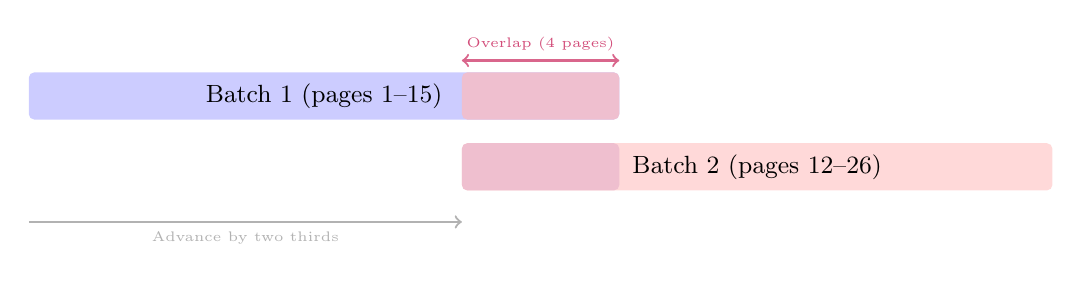
\begin{tikzpicture}
  % Batch 1
  \fill[blue!20, rounded corners=2pt] (0,0) rectangle (7.5,0.6);
  \node[font=\small] at (3.75,0.3) {Batch 1 (pages 1--15)};
  
  % Batch 2
  \fill[red!15, rounded corners=2pt] (5.5,-0.9) rectangle (13,-0.3);
  \node[font=\small] at (9.25,-0.6) {Batch 2 (pages 12--26)};
  
  % Overlap zone
  \fill[purple!25, rounded corners=2pt] (5.5,0) rectangle (7.5,0.6);
  \fill[purple!25, rounded corners=2pt] (5.5,-0.9) rectangle (7.5,-0.3);
  
  % Overlap label
  \draw[purple!60, thick, <->] (5.5,0.75) -- (7.5,0.75);
  \node[font=\tiny, purple!70, above] at (6.5,0.75) {Overlap (4 pages)};
  
  % Step arrow
  \draw[->, thick, gray!60] (0,-1.3) -- (5.5,-1.3) node[midway, below, font=\tiny] {Advance by two thirds};
\end{tikzpicture}
    \vspace{12pt}\caption{Overlapping window segmentation. Adjacent batches share boundary pages.}\label{fig:sliding_window}
\end{figure}

The design most important purpose is to preserve cross-boundary continuity: educational explanations that span a page break are captured intact in at 
least one complete batch, preventing the extraction model from receiving truncated input. This help greatly during graph construction when semantic overlap help knowledge 
island stay connected. As a small benefit to make up the overhead, the redundancy provides graceful degradation---if LLM encounter error when working with 1 batch, its overlapping 
neighbour still contains the boundary content, avoiding knowledge missing.

\subsubsection{Dual Phase LLM Extraction}\label{subsub:dual}

Dual Phase Extraction Pipeline is one that methodologically decouples top-down hierarchical decomposition from lateral relational mapping. Let $\mathcal{T}$ represent the continuous corpus of unstructured educational text, ingested from raw documents. The overall extraction objective is to discover an approximation function $\Phi: \mathcal{T} \rightarrow (V, E)$ that maximizes semantic fidelity. We decompose $\Phi$ into two sequential, deterministic mappings.
\begin{figure}[H]
    \centering
    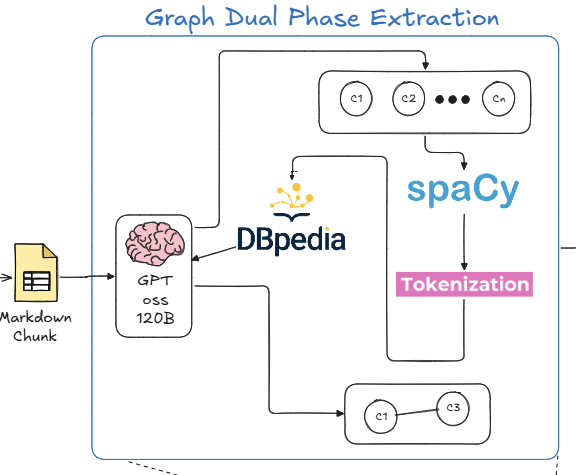
\includegraphics[width=0.65\textwidth]{Images/method/g_extract.png}
    \vspace{12pt}\caption{Dual Phase Extraction}\label{fig:g_ex}
\end{figure}
\subsubsection*{Phase 1: Top-Down Hierarchical Extraction (Skeleton Phase)}

The primary objective of the first phase is to establish the taxonomic structure of the knowledge domain without the cognitive burden of cross-referencing. The LLM's action space is strictly confined to identifying entities and their subsumption (parent-child) relationships.

We define the skeleton extraction function $\Phi_{\text{skeleton}}$ as:
\begin{equation}
    \Phi_{\text{skeleton}}: \mathcal{T} \rightarrow (V_{\text{tree}}, E_{\text{tree}})
\end{equation}
where $E_{\text{tree}} \subset V_{\text{tree}} \times V_{\text{tree}}$ contains strictly hierarchical edges (e.g., $ {PART\_OF}$).

To eliminate ontological drift, the LLM is forced to output data conforming to a rigid, predefined syntactic schema (e.g., strict JSON schema validation). The system parses this structural output to instantiate  {CommunityNode} and  {TopicNode} entities, ensuring that every atomic concept is firmly anchored to a macroscopic curriculum node.

Mathematically, this phase yields disjoint taxonomic trees. Because the LLM is only tasked with hierarchical assignment, the spatial complexity is bounded to $O(N)$ 
parent-child assignments. This drastic reduction in the problem space significantly mitigates the probability of generation errors. To complete the graph, phase 2 
is executed subsequently.

\subsubsection*{Phase 2: Lateral Relational Mapping (Relation Phase)}

With the hierarchical skeleton established as the logically structured frame, the second phase focuses on inferring the non-hierarchical, semantic linkages 
across different branches of the tree. Given the isolated, immutable entity set $V_{\text{tree}}$, the relational extraction function $\Phi_{\text{relation}}$ is 
defined as:
\begin{equation}
    \Phi_{\text{relation}}: (V_{\text{tree}}, \mathcal{T}) \rightarrow E_{\text{lateral}}
\end{equation}
where $E_{\text{lateral}}$ encompasses cross-cutting educational dependencies such as $ {PREREQUISITE\_OF}$ or $ {RELATED\_TO}$.

By presenting the LLM with a predefined, validated list of concepts ($V_{\text{tree}}$) and tasking it  {only} with edge generation, the problem space is reduced to a binary classification task over possible pairs. The final Educational Knowledge Graph is the formal union of these two sub-spaces: 
\begin{equation}
    G = (V_{\text{tree}}, E_{\text{tree}} \cup E_{\text{lateral}})
\end{equation}

To summarize, it is the operation of extracting potential candidate concepts as taxonomy trees and combine it to make a graph. This paradigm ensures high consistency 
in the generated graph. It bridges the gap between unstructured educational data and structured property graph by artificially 
constraining the LLM's action space, partlially preventing hallucinations. By partially, there is a big problem: Phase 2 relies mainly on Phase 1 for a structured and stable 
output, but what if Phase 1 itself is not a good frame skeleton? To better reconstruct and verify the frame, we use deterministic algorithm and techniques


\subsubsection{NLP-Based Concept Filtering and Verification}

The idea the Dual-Phase LLM Extraction (Section~\ref{subsub:dual}) is to reduces hallucination by constraining the model's action space of subsequent step using 
result from previous steps as an anchor and ground truth. However the raw output 
of Phase~1 remains inconsistence: semantically equivalent concepts may appear under distinct lexical forms, concepts extracted might not fit the full course content and
finally overly granular entities might be extracted just because it is mentioned once. In conclusion, using LLM to correct LLM has its limit. 
Inspired by BPE tokenization, a deterministic NLP pipeline is intergrated between Phase~1 
and Phase~2. This pipeline operates exclusively on the candidate node set $V_{\text{tree}}$ and produces a refined, verified set $V^{*} \subseteq V_{\text{tree}}$ 
that is subsequently passed to the Relation Phase. It is in fact a Entity Filterer proceeding through four sequential steps.

\paragraph*{Step 1 — Normalization and Tokenization.}

Each candidate concept label $v_i \in V_{\text{tree}}$ is first subjected to a standard text normalization procedure. This entails lowercasing, punctuation stripping, morphological lemmatization (reducing inflected word forms to their base lemma), and the removal of domain-agnostic stop words. The resulting form is then decomposed into a set of meaningful unigrams and bigrams, yielding a normalized token set $\mathcal{N}(v_i)$. Formally:
\begin{equation}
    \mathcal{N}(v_i) = \text{tokenize}\bigl(\text{lemmatize}(\text{lower}(v_i))\bigr) \setminus \mathcal{S}
\end{equation}
where $\mathcal{S}$ denotes the stop-word vocabulary. This normalization step establishes a canonical surface representation for every concept, ensuring that subsequent comparison operations are performed on semantically uniform token sets rather than raw, noisy strings.

\paragraph*{Step 2 — External Wiki Validation}

Following normalization, each candidate concept is submitted to the DBpedia Spotlight entity linking service. For a given concept $v_i$, the system issues a query against the DBpedia knowledge base to retrieve a set of $k$ candidate labels, denoted as $L_k$. 
To guarantee consistency and filter out unreliable terms, the system first identifies the most relevant label $l^*$ from the candidate set by maximizing the relevance score:
\begin{equation}
    l^* = \underset{l \in L_k}{\arg\max} \, \text{relevance}(l, v_i)
\end{equation}
Once the optimal label $l^*$ is identified, the concept is accepted and integrated into the knowledge graph only if this best match yields a positive relevance score:
\begin{equation}
    \text{relevance}(l^*, v_i) > 0
\end{equation}
If $\text{relevance}(l^*, v_i) = 0$, it indicates that even the most probable candidate of that entity definition yields no reliable definition on DBpedia. Concepts failing this 
criterion are usually either hallucinated constructs or excessively fine-grained pseudo-entities that lack grounding in established encyclopedic
 knowledge, and are subsequently pruned from $V_{\text{tree}}$. This external validation step introduces a strict layer of epistemic accountability, 
 anchoring the graph topology to verifiable, real-world semantics rather than model-generated approximations. 

 However, given the fact that todays researchers constantly discovering new paradigm and concepts that might have not been updated in Wiki, the system deliberately keeps 
 it as a Leaf Node with low weight. Though the node itself alone is not reliable, if its surrounding nodes are meaningful, its meaning can also be implicitly derived from 
 the graph structure, proposing a novel, robust architecture to new paradigm and innovation.
\paragraph*{Step 3 — Implicit Clustering}

Upon completion of filtering, the retained concepts undergo pairwise token similarity analysis. The Jaccard similarity between two concept representations is 
computed as:
\begin{equation}
    J(v_i, v_j) = \frac{|\mathcal{N}(v_i) \cap \mathcal{N}(v_j)|}{|\mathcal{N}(v_i) \cup \mathcal{N}(v_j)|}
\end{equation}

This measurement serves two complementary functions. First, concept pairs satisfying $J(v_i, v_j) \geq \tau_{\text{merge}}$ are treated as near-duplicates and 
consolidated into a single canonical node, thereby eliminating redundancy introduced by paraphrastic variation in the source text. Second, and more significantly, 
concepts that share a non-trivial common token subset — without necessarily crossing the merge threshold — are grouped into an  {implicit cluster}. The intersection 
$\mathcal{N}(v_i) \cap \mathcal{N}(v_j)$ is used to infer a shared parent topic label; for instance, the concepts ``Machine Learning Algorithms'' and ``Machine Learning Optimization'' 
both yield the shared token ``Machine Learning'', from which a  {TopicNode} bearing that label is derived. These implicitly discovered topic nodes are then cross-validated 
against the hierarchical skeleton produced by Phase~1 to either confirm existing  {TopicNode} entries or surface structural gaps in the original extraction.

\paragraph*{Step 4 — Node Caching.}

Once a concept node has successfully traversed Steps~1 through~3 — normalized, externally validated, and cluster-assigned — its canonical representation is persisted 
in a key-value cache, indexed by its normalized token set $\mathcal{N}(v_i)$. This cache serves three purposes. First, it ensures  {idempotency}: if the same concept surface form is encountered across multiple ingested documents, it resolves deterministically to the same canonical node without re-executing the NLP pipeline. Second, it supports  {incremental graph construction}: as new educational materials are added to the corpus over time, only genuinely novel concepts need to traverse the full verification pipeline, while previously verified nodes are retrieved directly from cache. Third, it provides the Relation Phase (Phase~2) with a stable, pre-validated entity vocabulary, eliminating the need for redundant lookups during edge generation. The final verified and deduplicated set $V^{*}$ is then passed forward as the immutable input to $\Phi_{\text{relation}}$.
\section{Teaching Assistance}
The knowledge graph $G$ serves as the static, structural foundation of the system. However, real-time interaction with a human 
learner demands a dynamic, adaptive reasoning engine capable of navigating $G$ to produce personalized educational responses. 
A single monolithic language model, no matter how capable, cannot reliably handle the diverse reasoning tasks involved in 
tutoring---from classifying student intent, to retrieving factual content with minimal cost and latency, to generating structured 
lectures, to evaluating learning outcomes. Each of these tasks requires a different workflow design.

To address this challenge, the proposed system decomposes the tutoring process into a multi-agent workflow, where each reasoning 
step is handled by a dedicated agent node with its own tailored prompt, tools, and output schema. The following subsections 
describe the core architectural decisions that make this decomposition both practical and effective: its applied harnessing 
as well as workflow design.

\subsection{Agent Harnessing}

Rather than relying on a single, prompt-heavy LLM to manage all tutoring logic, the Teaching Assistant is structured as a collection of specialized agent nodes 
coordinated through what we term an {Agent Harness}. This term was officially recognized worldwide this year, refering to all the infrastructure 
and pipeline revolves around the LLM. My proposed harnessing techniques govern how each node receives its instructions, what context it can access, 
and what format its output must follow. The design philosophy, from this point called the  {''Single Paradigm''}, is straightforward --- 
each agent node should have exactly one responsibility tied to one instruction set, one consistent context, and exactly one input/output structure/schema definition. 

\subsubsection*{Chat Summarization and Memory Management}

As a tutoring session progresses, raw chat history accumulates rapidly---exhausting the model's context window and degrading reasoning quality. The system addresses this with a sliding-window memorization mechanism: each turn is condensed into a structured triplet ( {query} $\rightarrow$  {thought} $\rightarrow$  {answer}), retaining only 8 entries at any time.

This history is exposed selectively: lightweight classification nodes (e.g., the intent router) receive only heading summaries ( {skim} mode), while nodes requiring deeper context---such as lecture generation or evaluation---receive the full summarized messages.

\subsubsection{Tool Abstraction Design}

Direct LLM access to the system's databases (Neo4j, Milvus, MongoDB, MinIO) risks malformed queries, unauthorized access, and destructive writes. A tool abstraction layer therefore sits between each agent and the underlying infrastructure: each tool exposes exactly one well-defined function, and agents have no direct access to raw query languages.

These tools are pre-configured with the student's session context before any agent invocation, making each call a simple, self-contained operation from the agent's perspective. This design simultaneously simplifies the agent's decision space and enforces strict data isolation across sessions.

\subsubsection{State---based Harnessing}

Even with many traditional context optimization techniques, agents still prone to context overhead when too many task instruction and tools metadata are injected, 
weaken their performance by miles and increase hallucination
The Dynamic Harness resolves this through state-dependent context injection: each workflow node receives its own dynamically populated prompt at runtime. 
Retrieval nodes get only retrieval-specific 
instructions; evaluation nodes receive evaluation criteria; synthesis nodes additionally receive upstream reasoning from prior nodes---yielding a minimal, 
purpose-built context window per node that collectively produces coherent multi-step reasoning.

Achieving this per-node dynamism requires intercepting agent execution at each workflow step---something standard frameworks (LangChain, CrewAI, AutoGen) do not 
natively support, as they fix agent configuration at initialization.
The solution proposed is the \textit{Adaptive Middleware}, which maintains an internal registry of workflow node names. When invoked at a node, it inspects the 
current node identifier, retrieves its registered harnessing protocol, and reconstructs the agent's configuration before execution.

\begin{figure}[H]
    \centering
    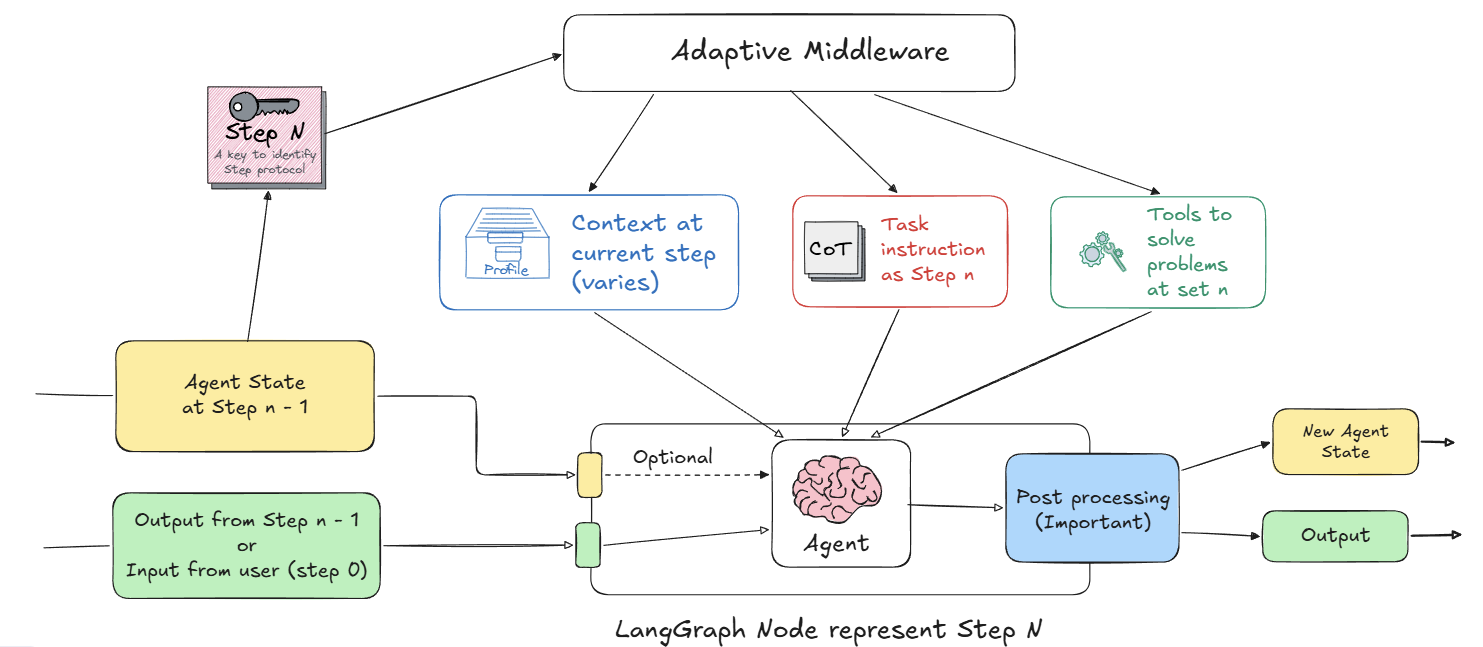
\includegraphics[width=1.0\textwidth]{Images/method/adaptive_middleware.png}
    \vspace{12pt}\caption{How agents's context and behaviour are constructed in a workflow node on a high level}\label{fig:agent2wf}
\end{figure}

This design offers 4 novel benefits:
\begin{enumerate}
 \item Single Paradigm is applied when a workflow node is registered with its own harnessing protocol, preventing the confusion that arises when a model must choose 
 among multiple possible reasoning paths, requirements, and methods.
 \item Because the middleware handles schema routing automatically, the prompt templates for each node can focus exclusively on the reasoning task at hand, without needing to include format-selection instructions.
 \item By constraining the output space to a predefined set, the system significantly reduces the probability of the model generating structurally invalid or semantically drifted responses. Each agent node operates within a tightly bounded action space---one task, one context, one schema---which collectively yields a more reliable and debuggable multi-step reasoning pipeline.
 \item With the registry techniques, agents are not hardcoded in nodes during initialization. This allows easy behaviour debug from the central registry, making agentic design more flexible and scalable.
\end{enumerate}

\subsubsection{Agentic Full Design}
Figure~\ref{fig:agent_harness} visualized a full harnessing of an agent, as well as its injection toward the workflow nodes to perform its task in a large 
LangGraph workflow, while table~\ref{tab:agent_tools} show us actionable protocols provided for agents in the form of Tools.

\begin{figure}[H]
    \centering
    \makebox[\textwidth][c]{
        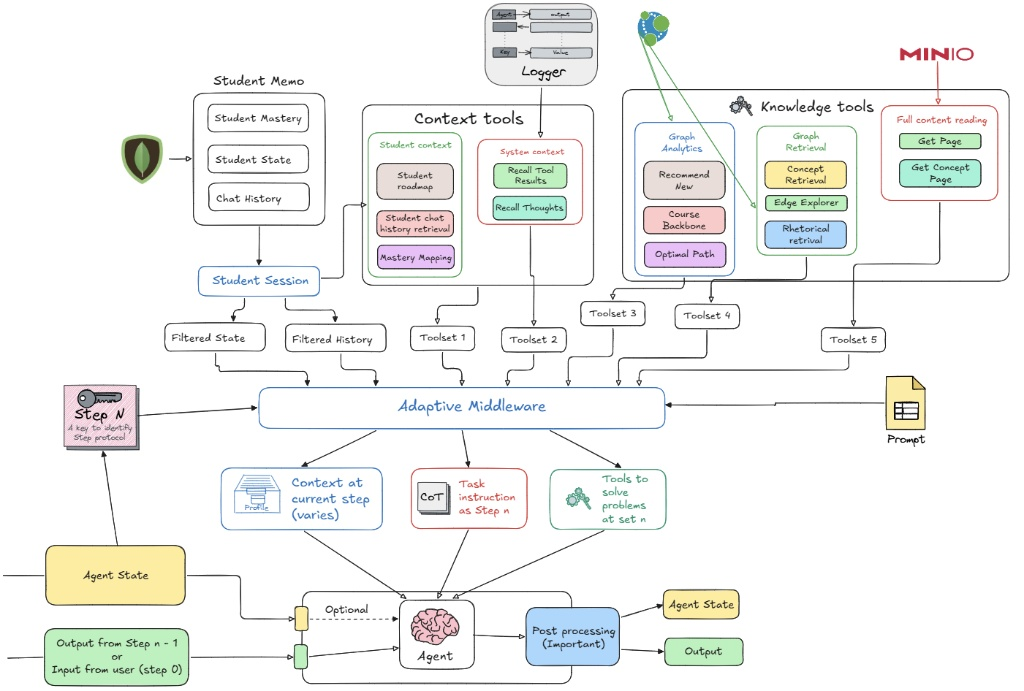
\includegraphics[width=1.1\textwidth]{Images/method/agent_design.jpg}
    }
    \vspace{12pt}\caption{Agent Harness architecture demonstrating the Adaptive Harnessing based on Middleware.}\label{fig:agent_harness}
\end{figure}

\begin{table}[H]
    \centering
    
    \renewcommand{\arraystretch}{1.3}
    \resizebox{\textwidth}{!}{
    \begin{tabular}{@{}llp{6.5cm}ll@{}}
        \toprule
        {Tool Name} & {Group} & {Description} & {Parameters} & {Database} \\
        \midrule
        \multicolumn{5}{@{}l}{{Context tools}} \\
        \midrule
        Student roadmap & Student context & Retrieve current student learning path and progress. &  {session\_id} & MongoDB \\
        Student chat history retrieval & Student context & Retrieve recent conversation history for context injection. &  {session\_id},  {limit} & MongoDB \\
        Mastery Mapping & Student context & Fetch student mastery scores for concepts. &  {session\_id} & MongoDB \\
        Recall Tool Results & System context & Retrieve recent tool execution results to prevent redundant calls. &  {limit},  {agent\_type} & Logger (In-memory) \\
        Recall Thoughts & System context & Retrieve recent agent reasoning traces for self-correction. &  {limit} & Logger (In-memory) \\
        \midrule
        \multicolumn{5}{@{}l}{{Knowledge tools}} \\
        \midrule
        Recommend New & Graph Analytics & Find top hub nodes ranked by out-degree for a starting point. &  {course\_filter},  {from\_node} & Neo4j \\
        Course Backbone & Graph Analytics & Extract course skeletal structure via top hub concepts and relations. &  {course\_name},  {max\_hubs} & Neo4j \\
        Optimal Path & Graph Analytics & Find the shortest weighted path between two concepts. &  {start\_node},  {end\_node} & Neo4j \\
        Concept Retrieval & Graph Retrieval & Resolve entity names to canonical IDs using graph or Wikidata. &  {query} & Neo4j \\
        Edge Explorer & Graph Retrieval & Explore multi-hop semantic relationships (excluding CONTENT edges). &  {node\_id} & Neo4j \\
        Rhetorical retrieval & Graph Retrieval & Retrieve educational content nodes by rhetorical role. &  {node\_id},  {role},  {limit} & Neo4j \\
        Get Page & Full content reading & Extract literal text from specific pages of a course document. &  {pages},  {destination} & MinIO \\
        Get Concept Page & Full content reading & Quickly locate page numbers referencing a specific concept. &  {concept} & Neo4j \\
        \bottomrule
    \end{tabular}
    }
    \caption{Summary of tools available to the Teaching Assistant agent.}
    \label{tab:agent_tools}
\end{table}

\newpage
\subsection{Agentic Workflow}

The Teaching Assistant's reasoning process is organized as a hierarchical state machine. At the top level, a router node classifies each incoming student query into 
one of five intent categories and dispatches it to the corresponding sub-workflow. Each sub-workflow is a directed graph of specialized nodes, where each node performs a single reasoning or data-retrieval step. Upon completion, every sub-workflow passes its results to a synthesis node that formats the final student-facing response and persists the session state. Figure~\ref{fig:smartedu} illustrates this top-level architecture.

\begin{figure}[H]
\centering
\begin{tikzpicture}[
  node/.style={rectangle, draw, rounded corners, minimum width=2.8cm,
               minimum height=0.7cm, font=\small, align=center},
  arr/.style={->, thick},
]

\node[node, fill=gray!20] (router) {TA\_Router\\{\tiny Intent Classification}};

\node[node, fill=green!15, below left=1.8cm and 0.4cm of router] (road) {WF\_Roadmap};
\node[node, fill=blue!15, left=0.6cm of road] (ret) {WF\_Retrieve};

\node[node, fill=orange!15, below right=1.8cm and 0.4cm of router] (teach) {WF\_Teach};
\node[node, fill=purple!10, right=0.6cm of teach] (prop) {Apply\_Proposal};

\node[node, fill=blue!8, below=1.5cm of ret] (retf) {TA\_Retrieve\_Finish};
\node[node, fill=green!8, below=1.5cm of road] (roadf) {TA\_Roadmap\_Finish};
\node[node, fill=red!10, below=4cm of router] (unk) {TA\_Unknown};
\node[node, fill=orange!8, below=1.5cm of teach] (teachf) {TA\_Teach\_Finish};

\node[node, fill=gray!30, below=7cm of router, minimum width=13.5cm] (end) {Session Context Saved\\(END)};

\draw[arr] (router) -- node[above left, font=\tiny, xshift=0.1cm] {retrieve} (ret.north);
\draw[arr] (router) -- node[left, font=\tiny, xshift=-0.1cm] {roadmap} (road.north);
\draw[arr] (router) -- node[right, font=\tiny, xshift=-0.1cm, yshift=-0.2cm] {unknown} (unk.north);
\draw[arr] (router) -- node[right, font=\tiny, xshift=0.1cm] {teaching} (teach.north);
\draw[arr] (router) -- node[above right, font=\tiny, xshift=-0.1cm] {confirm} (prop.north);

\draw[arr] (ret)  -- (retf);
\draw[arr] (road) -- (roadf);
\draw[arr] (teach) -- (teachf);

\draw[arr] (retf) -- (retf |- end.north);
\draw[arr] (roadf) -- (roadf |- end.north);
\draw[arr] (unk) -- (unk |- end.north);
\draw[arr] (teachf) -- (teachf |- end.north);
\draw[arr] (prop) -- (prop |- end.north);

\end{tikzpicture}
\vspace{10pt}
\caption{Top-level workflow routing based on user intents and context.}
\label{fig:smartedu}
\end{figure}

\subsubsection{Intent Router}

Every query must be dispatched to the correct sub-workflow before reasoning begins---misrouting wastes computation and produces structurally wrong responses. 
The router receives three inputs: (i) the student's current learning state, (ii) a  {skim}-mode chat summary, and (iii) the raw query---together disambiguating queries that appear identical but carry different intents across session contexts.

The prompting of the router goes for a straight forward {few-shot classification}: boundary-case examples for each routing choices. The output is a single constrained token 
from \{ {retrieve},  {roadmap},  {teaching},  {confirm},  {unknown}\} at temperature zero, with no tool invocation. This remove any time-cost reasoning chain, 
maximize speed and focus straight on real user input and well defined guildlines.

\subsubsection{Workflow: Roadmap}\label{subsub:wf_roadmap}

The Roadmap workflow addresses the planning problem:  {what should the student learn next, and in what order?} Unlike factual retrieval, this requires structural 
graph reasoning---the system must evaluate not only what exists in the knowledge base, but which concepts are most foundational, which the student has already 
mastered, and in what topological order they should be encountered. All structural analyses in this workflow consistently consider only semantic edges 
(prerequisite, hierarchical, associative) and explicitly exclude content-bearing edges, ensuring that centrality measures and path algorithms reflect 
presiquite dependency rather than rhetorical attachment.

\paragraph*{Out-Degree Centrality and Backbone Identification.}

The knowledge graph's density creates a navigation challenge---without a principled ranking, any learning path risks overwhelming the student or selecting concepts 
arbitrarily. The system addresses this with  {Out-Degree Centrality} as a structural heuristic. Heavily inspired by~\cite{DKG}, this is actually an algorithm to 
detect candidate central concept. Since the analytics is done on one type of edge, I propose a simplified version, ensured to be a built-in feature in Database. 
For a given node \(v\), the semantic out-degree \(C_{deg}(v)\) counts the number of outgoing semantic edges:

\begin{equation}
    C_{deg}(v) = \sum_{\substack{w \in V \\ (v,w) \in E_{\mathrm{sem}}}} 1
\end{equation}

where \(E_{\mathrm{sem}}\) excludes content-bearing edges. High-\(C_{deg}\) nodes serve as structural anchors and form the course backbone. 
This centrality measure is reused uniformly across all three sub-workflows: path planning (Roadmap), gap detection (Retrieve), and next-concept selection (Teach).

\paragraph*{Mastery State and the Knowledge Gap.}

The student's proficiency is represented as a  {mastery function} \(\mu : V \rightarrow [0, 1]\):

\begin{equation}
    \mu(v) =
    \begin{cases}
        s_v, & \text{if } v \in V_{\mathrm{explored}} \\
        0,   & \text{otherwise}
    \end{cases}
\end{equation}

where \(s_v \in [0,1]\) is the recorded Bloom's taxonomy mastery score for explored nodes, defaulting to zero otherwise. For any proposed backbone node \(b\), the set of unmastered prerequisites is:

\begin{equation}
    \Delta(b) = \{ u \in \mathcal{P}(b) \mid \mu(u) < \tau \}
\end{equation}

where \(\mathcal{P}(b)\) is the immediate prerequisite set of \(b\) and \(\tau\) is the mastery threshold. A non-empty \(\Delta(b)\) signals a knowledge gap that must be addressed before \(b\) is reachable.

\begin{figure}[H]
\centering
\begin{tikzpicture}[
  node/.style={rectangle, draw, rounded corners, minimum width=2.7cm,
               minimum height=0.8cm, font=\small, align=center},
  arr/.style={->, thick},
]
\node[node, fill=blue!15] (entry) {Entry Point:\\WF\_Roadmap};
\node[node, fill=cyan!10, right=1.5cm of entry] (explore) {Roadmap\_Explore\\{\tiny Pathway \& Hub Node Lookup}};
\node[node, fill=purple!10, right=1.5cm of explore] (eval) {Roadmap\_Evaluator\\{\tiny Feasibility vs Mastery Map}};
\node[node, fill=purple!10, below=1.2cm of eval] (advice) {TA\_Advice\\{\tiny Final Pedagogical Advice}};
\node[node, fill=gray!20, left=1.5cm of advice] (end) {Sub-graph END};

\draw[arr] (entry) -- (explore);
\draw[arr] (explore) -- (eval);
\draw[arr] (eval) -- (advice);
\draw[arr] (advice) -- (end);
\end{tikzpicture}
\vspace{10pt}
\caption{Roadmap sub-graph.}
\label{fig:roadmap_wf}
\end{figure}

Given the student's current position $v_{\mathrm{cur}}$, the system identifies the course backbone---its most foundationally connected concepts, ranked by $C_{deg}$---and computes the shortest prerequisite path to each backbone hub $b_i$ over the prerequisite sub-graph:
\begin{equation}
    \mathrm{Path}(v_{\mathrm{cur}},\, b_i) = [v_1, v_2, \ldots, v_k]
\end{equation}
These paths are merged and topologically sorted into a candidate list $\mathcal{L}$. To keep the result navigable, a sliding window retains only the top-$k$ nodes by $C_{deg}$ per segment $W_i \subset \mathcal{L}$:
\begin{equation}
    \mathrm{Selected}(W_i) = \operatorname{top\text{-}k}(W_i,\; C_{deg})
\end{equation}
yielding a condensed path where prerequisites always precede the concepts that depend on them:
\begin{equation}
    P_{\mathrm{roadmap}} = \mathrm{Selected}(W_1) \oplus \mathrm{Selected}(W_2) \oplus \cdots \oplus \mathrm{Selected}(W_m)
\end{equation}

Before the proposal reaches the student, it passes through a \textit{critic-actor} pass: a dedicated evaluator cross-references each backbone node against $\mu$, checking for unresolved gaps $\Delta(b) \neq \emptyset$, gatekeeper necessity, and cognitive load across the sequence. Its structured critique is then reconciled by an advisory agent into actionable guidance. Crucially, the resulting \textit{Learning Proposal} requires explicit student confirmation before modifying session state---unlike the auto-applied bridge proposals of the Retrieve workflow. Changing an entire learning trajectory is a high-stakes decision; the system is designed to inform and consent, not act unilaterally.

\subsubsection{Workflow: Retrieve}\label{subsub:wf_retrieve}

The Retrieve workflow answers factual questions by navigating the Educational Knowledge Graph. The workflow separates retrieval into two tiers---a fast, bounded lookup that satisfies most queries, and an optional deep structural analysis that activates only when a significant knowledge gap is detected.

\begin{figure}[H]
\centering
\begin{tikzpicture}[
  node/.style={rectangle, draw, rounded corners, minimum width=3.0cm,
               minimum height=0.8cm, font=\small, align=center},
  arr/.style={->, thick},
]
\node[node, fill=blue!15] (entry) {Entry Point:\\WF\_Retrieve};
\node[node, fill=cyan!10, below=1.2cm of entry] (core) {RAG\_Core\\{\tiny Global RAG \& KG Lookup}};
\node[node, fill=purple!10, below=1.2cm of core] (dec) {Deep\_Decision\\{\tiny Evaluate Gap Analysis}};
\node[node, fill=cyan!10, below left=1.2cm and 0.8cm of dec] (deep) {rag\_deep\\{\tiny Bridge Concept Retrieval}};
\node[node, fill=gray!20, below right=1.2cm and 0.8cm of dec] (end) {Sub-graph END};

\draw[arr] (entry) -- (core);
\draw[arr] (core) -- (dec);
\draw[arr] (dec) -- node[left, font=\tiny, xshift=-0.1cm] {\_deep\_route == 'deep'} (deep);
\draw[arr] (dec) -- node[right, font=\tiny, xshift=0.1cm] {\_deep\_route == 'skip'} (end);
\draw[arr] (deep) -- (end);
\end{tikzpicture}
\vspace{10pt}
\caption{Retrieval sub-graph. The flow routes dynamically to deep verification of prerequisite concepts if potential knowledge gaps are identified.}
\label{fig:retrieve_wf}
\end{figure}

The two-tier design reflects a deliberate efficiency-first principle: the majority of factual queries are definitional and can be resolved with a single graph traversal---resolving the concept to a canonical entity and fetching its rhetorical content (definition, formula, theorem, example). Forcing deep structural analysis on every query would inflate latency without benefit. A dedicated no-tool classifier therefore makes a binary routing decision after the initial lookup: simple queries exit directly to synthesis, while relational queries (\textit{how does X relate to Y}) activate the deep tier.

When deep analysis is triggered, the workflow shifts from content retrieval to \textit{structural gap bridging}: it traverses multi-hop semantic relationships to identify prerequisite nodes on the path between the student's current position and the queried concept, ranked by $C_{deg}$. A knowledge gap score $\gamma \in [0,1]$ quantifies the structural distance, and identified bridge concepts are packaged into a proposal that is applied automatically---reflecting the lower stakes of a targeted path adjustment compared to a full roadmap change.

\subsubsection{Workflow: Teach}\label{subsub:wf_teach}

The Teach workflow manages the continuous learning loop, delivering lectures, assessing mastery, and advancing the student's knowledge state through iterative interaction.

\begin{figure}[H]
\centering
\begin{tikzpicture}[
  node/.style={rectangle, draw, rounded corners, minimum width=3.0cm,
               minimum height=0.8cm, font=\small, align=center},
  arr/.style={->, thick},
]
\node[node, fill=blue!15] (entry) {Entry Point:\\WF\_Teach};
\node[node, fill=purple!10, below=1.0cm of entry] (und) {Teach\_Understand\\{\tiny Teaching Intent Classification}};
\node[node, fill=brown!10, below left=1.2cm and 1.8cm of und] (lkp) {Teach\_Lookup\\{\tiny Deterministic PDF Lookup}};
\node[node, fill=purple!10, below right=1.2cm and 1.8cm of und] (eval) {Teach\_Evaluate\\{\tiny Assess Learning Answers}};

\node[node, fill=cyan!10, below=1.2cm of lkp] (rag) {Teach\_RAG\\{\tiny RAG Fallback Query}};
\node[node, fill=orange!15, right=1.2cm of rag] (lec) {Teach\_Lecture\\{\tiny TA Lecture Generation}};
\node[node, fill=purple!10, below=1.2cm of eval] (nxt) {Next\_Topic\\{\tiny GraphDB Recommendation}};
\node[node, fill=gray!20, below=2.6cm of lec] (end) {Sub-graph END};

\draw[arr] (entry) -- (und);
\draw[arr] (und) -- node[left, font=\tiny, xshift=-0.1cm] {\_teach\_mode $\in$ ['continue', 'review']} (lkp);
\draw[arr] (und) -- node[right, font=\tiny, xshift=0.1cm] {\_teach\_mode == 'evaluate'} (eval);

\draw[arr] (lkp) -- node[left, font=\tiny] {source == NO\_CONTENT} (rag);
\draw[arr] (lkp) -- node[above, font=\tiny, yshift=0.1cm] {source == PDF} (lec);
\draw[arr] (rag) -- (lec);
\draw[arr] (eval) -- (nxt);

\draw[arr] (lec) -- (end);
\draw[arr] (nxt) |- (end);
\end{tikzpicture}
\vspace{10pt}
\caption{Teaching sub-graph flow: content lookup, RAG fallback, and adaptive topic progression.}
\label{fig:teach_wf}
\end{figure}

The central design philosophy is a \textit{Socratic loop}: deliver content, elicit a response, assess understanding, and either advance the student's position in the EKG or reinforce the current concept. A fine-grained entry classifier distinguishes three teaching modes---\textit{continue} (advance), \textit{review} (revisit), and \textit{evaluate} (assess)---ensuring the same surface query maps to the correct instructional behavior given the session state.

Content collection for lecture generation uses an iterative Reason-Act (ReAct) loop rather than a single retrieval call, allowing the agent to reason about what material is still needed and continue calling tools until the context $\mathcal{C}$ is sufficient (Figure~\ref{fig:react_teach}). Two tools drive this loop: \texttt{get\_concept} resolves the current node to a structured document reference (ID, MinIO path, page number), and \texttt{get\_pages} extracts the corresponding PDF pages; if no direct reference exists, the flow falls back to the Retrieve pipeline.

\begin{figure}[H]
\centering
\begin{tikzpicture}[
    node distance=1.4cm and 2.2cm,
    every node/.style={font=\small},
    startstop/.style={rounded rectangle, draw, fill=blue!8, minimum width=2cm, minimum height=0.7cm, align=center},
    action/.style={rectangle, draw, fill=green!8, minimum width=2.2cm, minimum height=0.7cm, align=center},
    decision/.style={diamond, draw, fill=orange!10, minimum width=1.2cm, minimum height=0.7cm, align=center, aspect=2.2},
    arr/.style={->, >=stealth, thick},
    darr/.style={->, >=stealth, thick, dashed}
]
    \node[startstop] (input) {Input Query};
    \node[action, right=of input] (context) {Context\\$C = [\text{input}]$};
    \node[decision, right=of context] (decide) {Sufficient?};
    \node[action, below=1.2cm of decide] (tool) {Tool Call:\\get material};
    \node[startstop, right=of decide] (output) {To Lecture\\Node};

    \draw[arr] (input) -- (context);
    \draw[arr] (context) -- (decide);
    \draw[arr] (decide) -- node[above] {\scriptsize Yes} (output);
    \draw[arr] (decide) -- node[right] {\scriptsize No} (tool);
    \draw[darr] (tool.west) -- ++(-1.8,0) node[midway, below, font=\scriptsize] {$C \leftarrow C \oplus \text{result}$} |- (context.south);
\end{tikzpicture}
    \vspace{12pt}\caption{ReAct loop in Teach Lookup.}\label{fig:react_teach}
\end{figure}

Lecture delivery is calibrated by the student's Bloom's taxonomy level: lower mastery receives definitions and grounded examples; higher mastery receives application problems and synthesis challenges. A closing challenge question is posed in \textit{continue} mode to close the teaching moment, while \textit{review} mode poses targeted recall questions over recently covered concepts. Assessment is deliberately tool-free---the agent judges mastery from conversational evidence alone, distinguishing genuine conceptual understanding from surface-level recall. The binary verdict then drives the session forward: a passing judgment triggers an auto-applied \textit{advance} proposal that moves the student's graph position to a high-centrality neighboring concept ranked by $C_{deg}$; a failing judgment returns a STAY action, preserving the current position for reinforcement.
